\section{Methods}
\label{sec:methods}

Before diving into the complex implementations and algorithms, it is essential that we visualize the core concepts mentioned in the previous section.

\begin{Note} 
    All of these visualizations are created using my own TypeScript implementation of a simple graphics library built on top of the HTML5 Canvas API. The code for this library is available in the repository of this thesis, and the visualizations can be viewed in the browser here: \url{https://kisskonraduni.github.io/emergent-animations/examples}.
\end{Note}

\vspace{0.2cm}

\subsection{Visualizing Coordinate Systems and Transformations}
\label{sec:visualizing-coordinate-systems}

Understanding how objects are positioned and transformed requires a clear grasp of the different coordinate spaces used in graphics programming.

From here on, I recommend opening the interactive examples on a nearby device, as the visualizations will be referenced throughout the thesis. While still images are provided for most examples, seeing them in motion is ideal. Let's begin by examining the main coordinate spaces used in graphics programming.

\Example{https://kisskonraduni.github.io/emergent-animations/examples/basics?tab=0}{Open interactive example}

\subsubsection{World Space}
\label{sec:world-space}

\begin{figure}[h]
    \centering
    \begin{minipage}[b]{0.4\textwidth}
        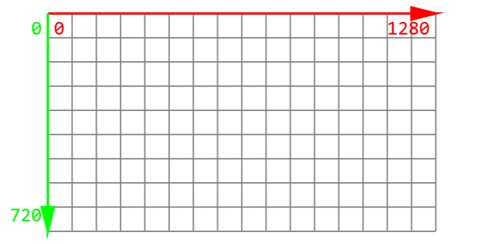
\includegraphics[width=\linewidth]{img/world-space.jpg}
        \caption{World Space Coordinate System \textbf{in my Graphics Library}}
    \end{minipage}\hfill
    \begin{minipage}[b]{0.55\textwidth}
        \setlength{\parskip}{1em}
        \setlength{\parindent}{0pt}
        World Space is the base coordinate system in a graphics library or game engine. The origin is at the top-left corner \textit{in my library}, with the x-axis pointing right and the y-axis pointing down. Almost all objects are positioned in this space, and transformations are applied relative to the origin.

        In this graphics library, I define a \(\vec{\text{resolution}}=[1280, 720]\) vector that represents the visible area.
    \end{minipage}
\end{figure}

\begin{Note}
    Technically speaking, the \(\vec{\text{resolution}}\) vector represents the bounds of an imaginary camera spanning from \([0, 0]\) to \([1280, 720]\). This variable is often used to define positions in the examples, as it makes our calculations easy to follow. The library ensures that, for any resolution and aspect ratio, this view is centered and fully visible on the screen.
\end{Note}

\pagebreak

\subsubsection{Object Space}
\label{sec:object-space}

\begin{figure}[h]
    \centering
    \begin{minipage}[t]{0.35\textwidth}
        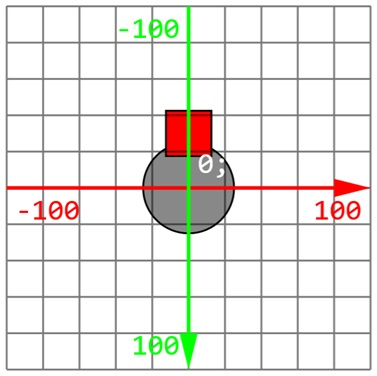
\includegraphics[width=\linewidth]{img/object-space.jpg}
        \caption{An example object with its Coordinate System visualized}
    \end{minipage}\hfill
    \begin{minipage}[b]{0.6\textwidth}
        \setlength{\parskip}{1em}
        \setlength{\parindent}{0pt}
        Object Space is the local coordinate system of an object, with the origin typically at the center. This space is used when defining the object's geometry and rendering. Transformations in Object Space are applied relative to the object's pivot point.

        The object has a tiny hat as a child element to visualize the local coordinate system. The hat's position is set relative to the circle's pivot point and moves with it. If we want the hat's position in World Space, we need to apply the object's transformations to the vector representing the hat's position.
    \end{minipage}
\end{figure}

\begin{Note}
    The pivot point is the reference for rotation and positioning within World Space. Correctly setting the pivot point is crucial: for UI elements, it allows easy anchoring; for game objects, such as a player character, the pivot is often set to the feet to ensure rotation occurs around the correct point.
\end{Note}

\vspace{1cm}

\subsubsection{Screen Space}
\label{sec:screen-space}

In this graphics library, Screen Space typically matches World Space, with the origin at the top-left corner. In 3D applications, an additional Camera Space is introduced: World Space $\rightarrow$ Camera Space $\rightarrow$ Screen Space. Camera Space represents the camera's position and orientation, while Screen Space is where the camera's view is projected, either at the top-left or center of the screen. This separation is important, as game objects and UI elements often exist in different spaces or layers.

\begin{Note}
    Using these transformations, we can create interactions between different spaces. For example, dragging an object in Screen Space can be transformed into World Space to update its position. Most 3D editors use a similar approach. This is possible because transformations can be inverted, allowing us to transform a point from Screen Space to World Space, or from Object Space to World Space.
\end{Note}

\pagebreak

\subsection{Understanding "Objects" in Graphics Programming}
\label{sec:understanding-objects}

In graphics programming, the term "object" can refer to various entities, from simple shapes to complex models. The key to animating these is understanding their properties and how we can build our scenes using them.

\Example{https://kisskonraduni.github.io/emergent-animations/examples/basics?tab=1}{Open interactive example}

\subsubsection{Basic Properties}

There are a few properties that most implementations use to define objects:

\begin{itemize}
    \item \textbf{Position:} The object's position, typically represented as a vector.
    \item \textbf{Rotation:} The object's orientation, often represented as an angle in 2D, as a 3D vector using Euler angles in three dimensions, or as a quaternion in more advanced implementations. See \cite[Section~10.6]{learn-opengl} for more information.
    \item \textbf{Scale:} The object's scale is a vector that defines how much the object is stretched or compressed in each dimension. Note that scale does not directly represent the object's size, but rather its proportional transformation along each axis.
    \item \textbf{Parent:} The object's parent, if defined, is another object that serves as the basis for its transformations. Circular dependencies and self-references are not allowed.
\end{itemize}

Notably, these properties do not explicitly define a coordinate system; instead, they are always interpreted in the parent object's Object Space, or in World Space if no parent exists.

\Example{https://kisskonraduni.github.io/emergent-animations/examples/basics?tab=2}{Open interactive example}

An emergent behavior of these properties is that we can create complex animations with simple parent-child relationships.

\vspace{0.5cm}

\subsubsection{Drawing Objects}

Drawing an object typically involves rendering its geometry, which can be as simple as a circle or as complex as a 3D model. A key aspect of this is that we define a \textbf{size} property for the object, which is \textbf{not} the same as the scale property. 

The size is used to determine how large the object appears on the screen, while the scale is used to stretch or compress the object in its Object Space. As an extra note, the way we position the object before drawing is also important, usually defined by another property called the \textbf{pivot point}. For an explanation, see \ref{note:6}

\pagebreak

\begin{Note}
    The size property often can be an implied property from the data we use to define how we draw said object. For example, a 3D model would be defined by points in space around the origin, and the size would be the distance between the furthest points in each axis.
\end{Note}

The exact implementation used to draw the object depends on the graphics library or engine, so I will not go into detail here, as it is not the focus of this thesis. However, I will outline the general steps taken, as it is important to understand how these objects are rendered:

\begin{itemize}
    \item \textbf{Apply the transformation stack.} - Get all the elements in the transformation stack, and "apply" them in the order they were added.
    \begin{Note}
        "Applying" the transformation stack can differ depending on the implementation. Most commonly, this means multiplying the current transformation matrix by the transformation matrix of the object. The starting "World Space" matrix is the identity matrix, which represents no transformation. The order of multiplication matters, as it determines how the transformations are applied.
    \end{Note}

    \item \textbf{Draw the object.} - Use the current transformation matrix to draw the object in its Object Space, using its size and pivot point.

    \item \textbf{Reset the transformations for the next object.} - After drawing the object, reset the transformations in order to avoid affecting subsequent objects.
\end{itemize}

Take this method and repeat it for every object in the scene. An extra caveat in 2D is that draw order matters (sometimes it matters in 3D as well, but that is not the focus of this thesis), so we need to make sure that the objects are drawn in the correct order. We can imagine them as stickers being placed on top of each other, where the last sticker drawn is the one on top. This is why we often use a "z-index" property to determine the order of drawing if we do not want to manually sort the objects.

\pagebreak


